% !TeX encoding = UTF-8
% !TeX root = ../main.tex
% !TeX spelling = en_GB
% !dsfaTeX program = latexmk

\chapter{Theory}
\label{chap:theory}

This chapter begins with an introduction to the physics behind the forming of ice on structures. The next two sections briefly describe the measurement parameters and some practical problems of measuring icing. The last section is about scattering of light by small particles.

\section{Forming of Ice}

Cold climate areas, according to the definition by IEA \cite{iea2017} are regions that experience frequent atmospheric icing or periods with temperatures below the operational limits of standard IEC 61400-1 ed3
wind turbines. Atmospheric icing is the period of time where atmospheric conditions are present for the accretion of ice or snow on structures \cite{iea2017}.

An icing event can be divided into three phases: the incubation, the accretion and the persistance/ablation. Meteorological icing, which is the main interest of this thesis, is the period during which the meteorological conditions (temperature, wind speed, liquid water content, droplet distribution) allow ice accretion. The incubation is the time in meteorological icing before the accretion starts. The length of each of these phases, and the severeness of the icing depends on a combination of the aerodynamic shape and temperature of the structure or airfoil, the velocity of the air and its contained water, the air temperature, the mixing of snow and water, the concentration of liquid water and the droplet size distribution.

Wheather a particle is likely to follow the flow or collide depends on the flow velocity, the size and shape of the obstacle and the density and drag coefficient of the particle. This relationship is known in fluid mechanics as the Stokes number ($Stk$). Small droplets or particles with $Stk \ll1$ may continue with the airflow around the profile, while large droplets or particles with $Stk \gg 1$, due to their inertia, collide with the structure. A supercooled droplet colliding with a structure is likely to freeze upon impact. Figure \ref{fig:freezedrops} illustrates the difference between large and small supercooled droplets passing an aerodynamic profile.

\begin{figure}%[h]
\centering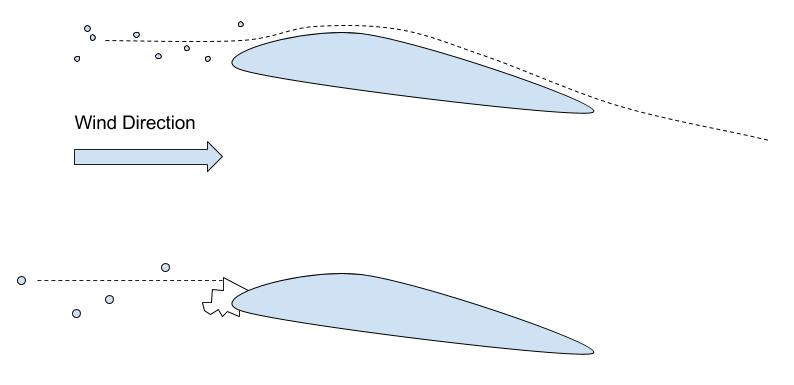
\includegraphics[width=0.8\linewidth]{./figures/freezing_droplets.jpg}
\caption{Supercooled water droplets on collision course with an aerodynamic profile.}
\label{fig:freezedrops}
\end{figure}

Icing on wind turbines forms slightly differently from ice accretion on an aircraft airfoil. Unlike aircrafts, the turbine is stationary and cannot stop the icing, or de-ice by moving to a different position. The same conditions may persist for days or weeks. The turbine blade moves concentrically making the tip of the blade the fastest, and highest located moving part. There is no status surveillance of the wings. Therefore the remote and exposed position makes it difficult to detect ice directly when it is initially formed \cite{homo2006}.

\section{Liquid Water Content and Median Volume Diameter}

The liquid water content (LWC) and the water droplets median volume diameter (MVD) are parameters that can be used to predict or model icing. The  MVD is given at the point where half of the total volume of liquid content in a fixed air volume consists of droplets with larger diameters, and half with smaller diameters. The MVD has been assumed to give the best approximation to the spectrum of diameters in a droplet distribution, when considering the collision efficency \cite{fins1988}. To estimatie the amount of icing created by supercooled water droplets, the MVD has been shown to be a good indicator in most cases \cite{makk2000}. The MVD as approximation to the distribution of diameters can be used to simulate ice accretion on wind turbines \cite{dier2011}.

In practice, the LWC and MVD are rarely measured at a planned or existing wind turbine \cite{parent2011, makk1992}. Measuring these properties accurately and frequently would be an advantage for the planning of new wind mill farms or for the application of anti-icing arrangements on existing power stations. It may be of particular interest as input to weather prediction models, by which both LWC and MVD can be computed \cite{thomp2009, nyga2011}. In combination with information about the aerodynamic properties of the wind turbine, it can give more accurate predictions of icing or even result in better design of wind turbines and anti-icing methods.

While icing caused by large supercooled droplets, with diameters from approximately 50 μm to more than 1000 μm, is often considered severe due to its shape and quick build-up, icing may occur even with droplets as small as 5 μm \cite{sand1984, cob2001, homo2010}. In most cases though, icing is caused by cloud droplets measuring between 10 μm and 30 μm in diameter \cite{makk1992, cob2001}.

Although optical imaging and other techniques for measuring aerosol properties are continuously improving, the choice of instrument is still very much dependent on the application’s requirements \cite{ide1999, baum1983, baum2011, kulk2011}. An instrument for measuring icing parameters for wind turbines should be able to detect supercooled cloud droplets as small as five micrometer and determine an accurate measure of LWC. Since measurements are needed in multiple remote locations, it should also be affordable, reliable, have low power consumption, and, ideally it should be possible to place it near the highest point of the turbine \cite{homo2006}.

\section{Practical Problems with Measuring Atmospheric Water}

The varying nature of atmospheric water particles mentioned in the previous chapter makes it very difficult to measure all kinds and sizes of particles using a single instrument. Therefore, atmospheric aerosol studies are often done with one or several instruments combining different techniques. Each technique with its own limitations and problems. It is also difficult to find a reference sample with the same but known properties as the water. Free floating water droplets are affected by gravity, they eventually collide and coalesce, evaporate or stick to adjoining  surfaces. This makes it difficult to measure and find out the physical properties without affecting the sample.

The size of water droplets range from a few micrometers to several mm in diameter. An imaging instrument is limited by the optical system's resolution, its field of view and the usable depth of field or the measuring range.

Many existing instruments suffer from errors caused by the instrument itself during sampling, e.g. when droplets get stuck on the inlet \cite{spie2012}. At higher wind speeds particles shatter into smaller droplets or bounce on the supporting structure making up the instrument \cite{cohen1991,field2006}. All droplets or particles approaching an obstacle are affected by the change in pressure and wind direction surrounding it, a fact which complicates measuring the concentration of particles in unaffected air. Measurement probes working by extraction of air using a mechanical air pump would expect a loss of particles with large Stokes numbers. Ideally, the measuring device should be designed to have as little effect on the free flow of particles as possible \cite{baum2011}.

An example of an instrument that makes use of the fact that supercooled water droplets will freeze upon impact, is the rotating cylinders used by Makkonen \cite{makk1992}. By exposing cylinders of different diameters, depending on the amount of ice accumulated on each cylinder, the MVD and LWC can be calculated using a theoretical model. While this technique provides an alternative to the single particle measurements its drawback is that it requires a certain extent of manual operation, in addition to the fact that only freezing water can be measured.

Measuring particles via aircraft is complicated by the high air speed. The sample is affected by the change in pressure surrounding the aircraft and by particles hitting parts of the probe, splintering or changing direction, causing anisokinetic sampling \cite{baum2011}. An instrument fixed to the ground on the other hand is affected by the wind speed relative to the ground. This means that it needs to be directed in the direction of the wind. Particles may also enter the measurement zone from different directions depending on their Stokes number, which has been shown to have an effect on the measured liquid water content \cite{henn2013}.

Instruments based on Mie calculations of light scattering sometimes struggle to deal with with a non-linear relation between scattering response and diameter. Aliasing in the sample bin resolution can lead to spikes in the size distribution. Particularly interesting is the 10 to 15 μm range, where two particles with diameters differing more than one micrometer can have the same scattering intensity response \cite{dye1984,spie2012,bohr2008}.

\section{Light Scattering and Absorption}

In visible light, water is almost transparent. This means that the imaginary part of the refractive index, i.e. the absorption, is very small, while for some wavelengths it increases many times. This fact is used in two-color lidar measurements \cite{west2010}. The real part of the refractive index for water is much more stable; approximately 1.3 in the visible to near infrared range \cite{hale1973, kou1993}. 

For a shadowgraph system, it is possible to assume that the refractive index of air is equal to one. A droplet works as a spherical lens with a very short focal length. Exposed to a background illumination it will scatter almost all of the light that reaches the droplet, causing a shadow that appears as a black disc except for the light passing straight through the center. Some of the light will also be absorbed, even if the absorption of a single water droplet is negligible, due to its small volume and water absorbing very little in the visible spectrum.

When the light source is large compared to the size of the droplets, as in the case of using a collimated LED, the intensity of the center Arago spot caused by Fresnel diffraction is be negligible \cite{reis2017}.

The combined effect of scattering and absorption is the extinction \cite{bohr2008}. Due to this combined effect, clouds look nontransparent from a distance. Measuring extinction is possible in aerosols, e.g. by using Raman LIDAR \cite{ans1990}.

